\subsubsection{1.4. Các mô hình GNN Baseline}
\indent\indent Đề tài thực hiện xây dựng và huấn luyện 5 mô hình mạng nơ-ron đồ thị cơ sở bao gồm: GATv2, GCN, GINE, PNA và Graph Transformer. Mục tiêu của bước này là tạo ra một mốc tham chiếu để đánh giá khả năng học đặc trưng đồ thị với các cơ chế truyền tin khác nhau, đồng thời cung cấp vector embedding cho giai đoạn phân loại nâng cao phía sau.\vspace{0.3cm}

Kiến trúc tổng quát của các mô hình GNN baseline được minh họa tại \textbf{Hình \ref{fig:GNNArchitecture}}, tuân thủ luồng xử lý đồng bộ để đảm bảo tính công bằng trong thực nghiệm:\vspace{0.3cm}

\begin{figure}[H]
    \centering
    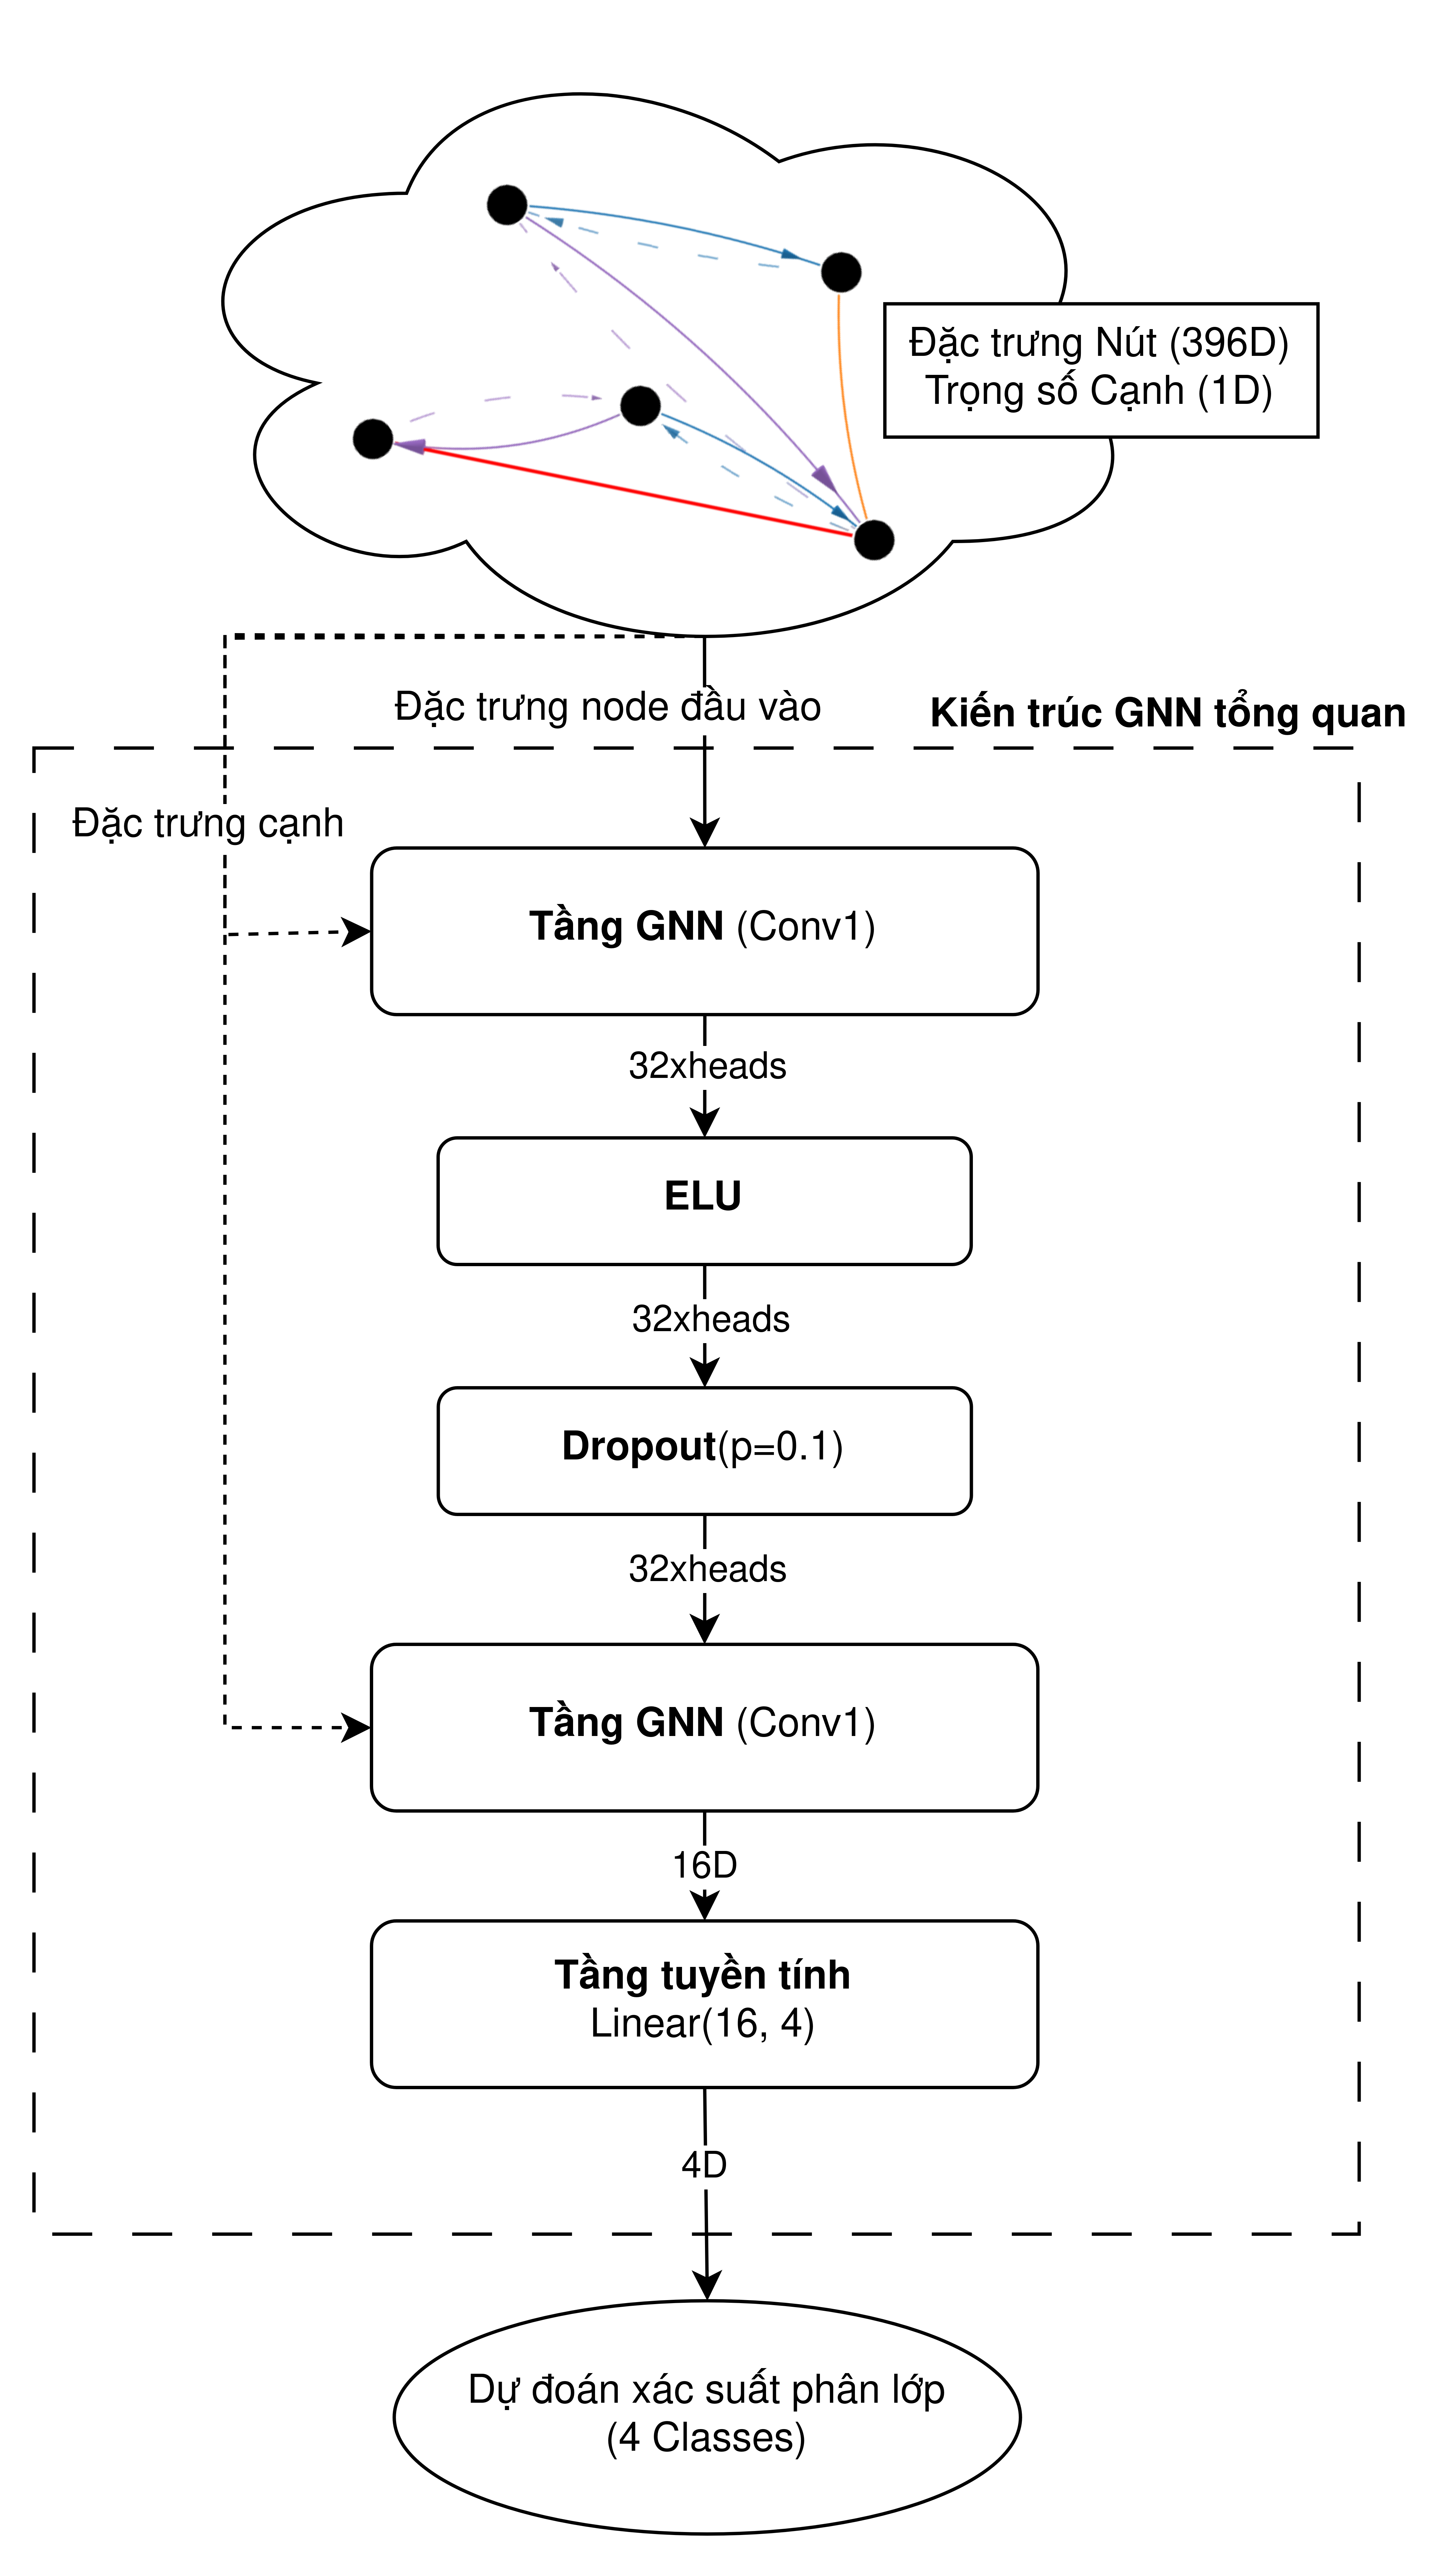
\includegraphics[width=0.55\linewidth]{images/part-02/chap-02/sec-01/GNNArchitecture.png}
    \vspace{0.2cm}
    \caption{Kiến trúc tổng quan của các mô hình GNN Baseline}
    \label{fig:GNNArchitecture}
\end{figure}

\textit{1.4.1. Đặc tả dữ liệu đầu vào và đầu ra}

\begin{itemize}[label={--}, itemsep=3pt]
    \item \textbf{Đầu vào:} Dữ liệu đồ thị bao gồm ma trận đặc trưng nút $X$ ($396$ chiều) và các thuộc tính cạnh đại diện cho trọng số hành vi $w_{ij}$.
    \item \textbf{Đầu ra:} Kết quả dự đoán xác suất cho 4 lớp đối tượng: \texttt{BENIGN}, \texttt{LOW\_RISK}, \texttt{HIGH\_RISK} và \texttt{MALICIOUS}.
\end{itemize}

\textit{1.4.2. Quy trình xử lý}\vspace{0.2cm}

\indent Quy trình xử lý của các mô hình baseline được chia thành hai giai đoạn chính nhằm tối ưu hóa việc trích xuất tín hiệu từ đồ thị thưa thớt:

\begin{itemize}[label={--}, itemsep=3pt]
    \item \textbf{Giai đoạn trích xuất đặc trưng:} Hệ thống sử dụng cấu trúc hai tầng tích chập đồ thị (\textit{Message Passing}) để khai thác thông tin cấu trúc:
    \begin{itemize}[label={+}, itemsep=2pt]
        \item \textbf{Tầng mở rộng (Layer 1):} Chuyển đổi từ 396 đặc trưng thô sang không gian ẩn trung gian (32 đơn vị × số đầu chú ý). Tại đây, hàm kích hoạt ELU và Dropout (0.1) được áp dụng để ổn định tín hiệu và chống quá khớp.
        \item \textbf{Tầng nén đặc trưng (Layer 2):} Toàn bộ các mô hình đều được ép về một không gian 16 chiều. Vector này đóng vai trò là thông tin tổng hợp tinh túy nhất về hành vi của một nút.
    \end{itemize}
    \item \textbf{Bộ phân lớp (Linear Classifier):} Sử dụng một tầng tuyến tính (\textit{Fully Connected}) để ánh xạ vector biểu diễn 16 chiều thu được từ tầng nén sang không gian nhãn mục tiêu.
\end{itemize}

\textit{1.4.3. Đặc thù cấu hình các biến thể kiến trúc}\vspace{0.2cm}

\indent Mặc dù cùng tuân thủ khung kiến trúc chuẩn, mỗi biến thể GNN được tùy chỉnh cơ chế truyền tin để xử lý trọng số cạnh $w_{ij}$ theo các phương pháp đặc thù:
\begin{itemize}[label={--}, itemsep=3pt]
    \item \textbf{GATv2 \& Transformer:} Sử dụng cơ chế chú ý động với 4 đầu chú ý độc lập, tích hợp $w_{ij}$ trực tiếp vào quá trình tính điểm chú ý.
    \item \textbf{GCN:} Tiếp nhận $w_{ij}$ dưới dạng \texttt{edge\_weight} để điều chỉnh cường độ lan truyền tin nhắn một cách trực tiếp dựa trên cấu trúc đồ thị.
    \item \textbf{GINE:} Sử dụng mạng nơ-ron đa tầng nội tại để nhúng trọng số cạnh vào thông điệp của láng giềng trước khi thực hiện phép cộng.
    \item \textbf{PNA:} Áp dụng ghép nối $w_{ij}$ vào đặc trưng láng giềng thông qua tầng tiền xử lý $MLP_{pre}$. Điều này giúp 4 chỉ số thống kê (đặc biệt là độ lệch chuẩn $\sigma$) định lượng trực tiếp sự biến thiên của cường độ hành vi.
\end{itemize}